\chapter{Ukázka práce}

Výsledkem této práce je tedy implementace systému pro porovnávání výkonu verzí softwaru
pojmenovaný PerfEval. V této kapitole bude krok za krokem ukázáno, jak se systémem pracovat.

\section{Používání systému PerfEval}

V~následujícíh dvou ukázkách bude vysvětleno, jak používat PerfEval. První ukázka bude
cílit na nastínění, co+nejjednoduššího použití. Druhá se bude snažit o~složitější použití
systému PerfEval.

\subsection*{Jednoduché použití PerfEvalu}

Následující kód popisuje obvyklou posloupnost příkazů práce se systémem PerfEval.
Na začátku je nutné jej inicializovat. PerfEval bude inicializován pro použití JMHJSONParseru.
Následně se přidají výsledky měření několika (alespoň dvou) různých verzí.
Nakonec program vypíše jestli výkonnostní testy prošly, nebo ne.

\begin{lstlisting}
    perfeval init --benchmark-parser JMHJSONParser
    perfeval index-all-results --path path/to/dir/with/results --version x.y.z
    perfeval index-all-results --path path/to/another/dir/with/results --version x.y.z2
    perfeval evaluate && echo "Performance test passed" | exit 0
    echo "Performance test failed" | exit 1
\end{lstlisting}

\subsection*{Návrh skriptu pro doměření výsledků}

Následující kód nastiňuje možnost využití příkazu list-undecided. Výstupem tohoto příkazu
jsou dva tabulátorem oddělené sloupce. V prvním sloupci jsou názvy metod, pro něž systém
eviduje málo naměřených běhů. Ve druhém sloupci je uveden tento počet. Příkaz je určený
pro skriptování, proto není dodaná žádná další hlavička.

V případě, že výstupem není žádný výpis, tak je hodnot u všech testovacích metod naměřeno dostatek. Druhou alternativou
je, že v důsledku nastavení v~konfiguračním souboru systém vyhodnotil, že není možné požadovaný
počet testů doměřit. Následné vyhodnocení pak bude vyžadovat kontrolu uživatelem, Protože
systém PerfEval bude vyhodnocení považovat za nevyhovující.

Skript projde všechny řádky výpisu. Pokud je výpis prázdný, tak skončí.
V~následujícím kódu je celá situace velmi zjednodušena. Nalezene se maximální počet
testů, který je zapotřebí změřit. Pro~tento maximální počet se změří výkony obou verzí znovu.
Tudíž může dojít i~k~měření pomocí metod, které nejsou zapotřebí. Výsledky těchto měření
se zaznamenají do~systému PerfEval. Po~doběhnutí všech měření skript skončí. Vyhodnotí mezi sebou výsledky těchto
verzí a~skončí. Parametry \$1 a~\$2 jsou stará a~nová verze k~porovnání. Předpokládá se, že
příkaz measure provede měření verze zadané jako první argument a~výsledek uloží do souboru specifikovaného jako druhý argument.

\begin{lstlisting}
    #!/bin/bash

    # Function to find the maximum value in the second column
    find_max() {
        max=0
        while IFS=$'\t' read -r _ val; do
            if [[ $val =~ ^[0-9]+?$ ]]; then
                if (( $(echo "$val > $max" | bc -l) )); then
                    max=$val
                fi
            fi
        done
        echo "$max"
    }

    # Main script
    index=1
    while true; do
        output=$(perfeval list-undecided --old-version "$1" --new-version "$2")
        if [[ -n "$output" ]]; then
            max=$(echo "$output" | find_max)
            for ((i=1; i<=$max; i++)); do
                result_file="old_version_$index"
                measure "$1" "$result_file"
                perfeval index-new-result --path "$result_file" --version "$1"

                result_file="new_version_$index"
                measure "$2" "$result_file"
                perfeval index-new-result --path "$result_file" --version "$2"
                ((index++))
            done
        else
            perfeval evaluate --old-version "$1" --new-version "$2"
            exit $?
            break
        fi
    done

\end{lstlisting}

\section{Nasazení systému v praxi}

Pro prezentování fungování PerfEvalu s reálnými daty jsem si vybral softwarový projetk crate.
Tento projekt je dostupný na GitHubu (\cite{crateDB}) a jeho autoři používají k vyhodnocování výkonu framework JMH.
Pomocí testů od autorů bylo provedeno měření několika verzí. Byly vybírány zejména verze jejichž
commit message se zmiňovala o zlepšení výkonu a verze před tímto zlepšením.

Projekt byl z~výše zmíněného Githubu naklonován do~lokálního adresáře. Následně došlo
k~nalezení commitů u~nichž zpráva tvrdí, že~došlo k~výraznému zlepšení výkonu.

\begin{lstlisting}
commit b838a4ac7dd37f85a3b5ea2ae2c1b3040fb08929
Author: Andrei Dan <andrei@crate.io>
...skipping...
    using DocValues over source lookup will greatly increase performance.
    the reasons for doing a source lookup instead were mostly related to the
    pre-DocValues era were the fieldcache was used instead.

commit 968a5fcae558f904fb2ebdc747bae1dadc567cfb
Author: Sebastian Utz <su@rtme.net>
Date:   Fri Jan 12 12:37:58 2018 +0100

    re-enables StringTypeTest JMH benchmark by moving it to benchmarks module

    was a left over from the recent JMH benchmarks refactoring

\end{lstlisting}

U obou verzí došlo měření výkonu. Měření projektu jsou součástí projektu, takže došlo
pouze ke~spuštění JMH testů a~uložení výsledků ve~formátu JSON. Po naměření byly porovnány
výše uvedené verze.

\begin{figure}[h!]
    \centering
    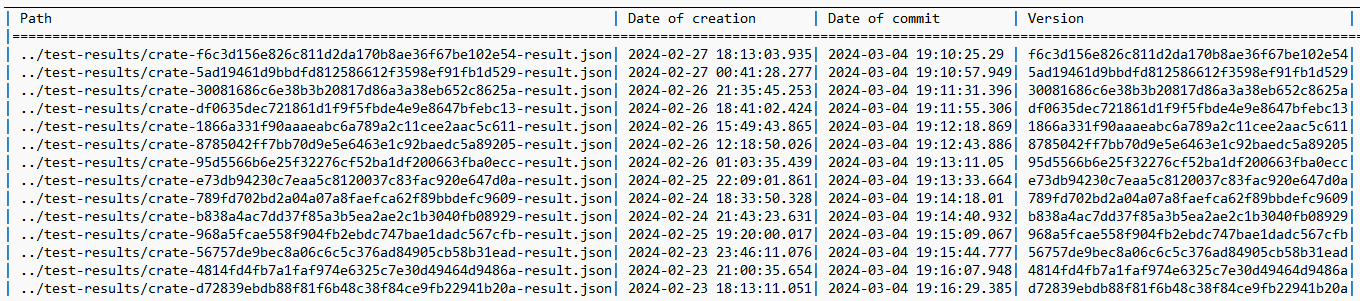
\includegraphics[width=1\textwidth]{../img/list-results-crate.png}
    \caption{Obsah databáze systému PerfEval pro projekt crate}
\end{figure}

\begin{figure}[h!]
    \centering
    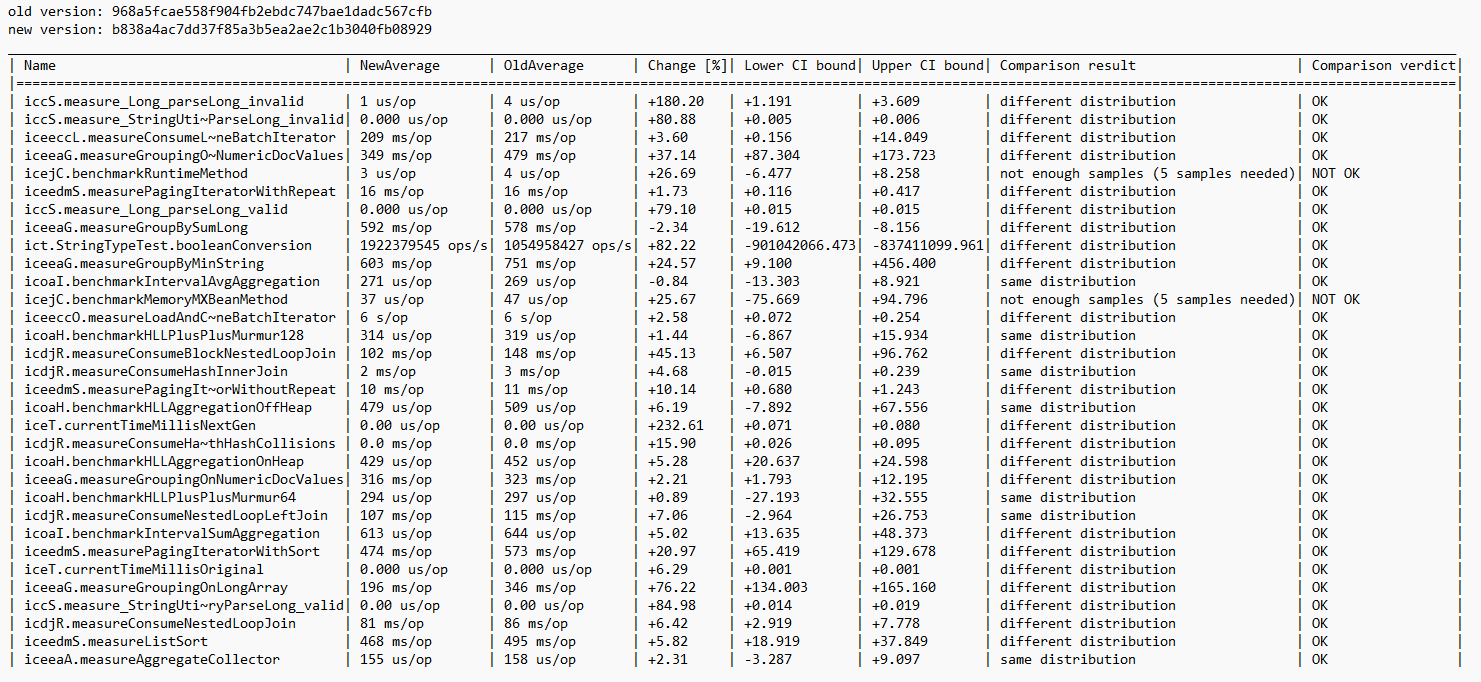
\includegraphics[width=1\textwidth]{../img/version-comparison-nes.png}
    \caption{Výsledek porovnání mezi commity}
\end{figure}

Z~výsledků porovnání je vidět, že došlo k~nějakému zlepšení výkonu. I přes to, že
ve dvou případech došlo ke zlepšení v řádu stovek procent, tak test selhal s~kódem 1.
Toto selhání je zapříčiněno přísliš malým počtem změřených běhů pro dvě měřené metody.
Jedná se o~metodu benchmarkRuntimeMethod a~o~metodu benchmarkMemoryMXBeanMethod.

V~důsledku malého počtu změřených běhů bude měření dalších běhů simulované. Nové
výsledky měření budou simulovány tak, že se již přidané soubory s výsledky přidají vícekrát.
Toto vícenásobné přidání se projeví v databázi PerfEvalu obsahující informace o~výsledcích měření tak,
že se zde stejný řádek bude vyskytovat vícekrát.

\begin{figure}[h!]
    \centering
    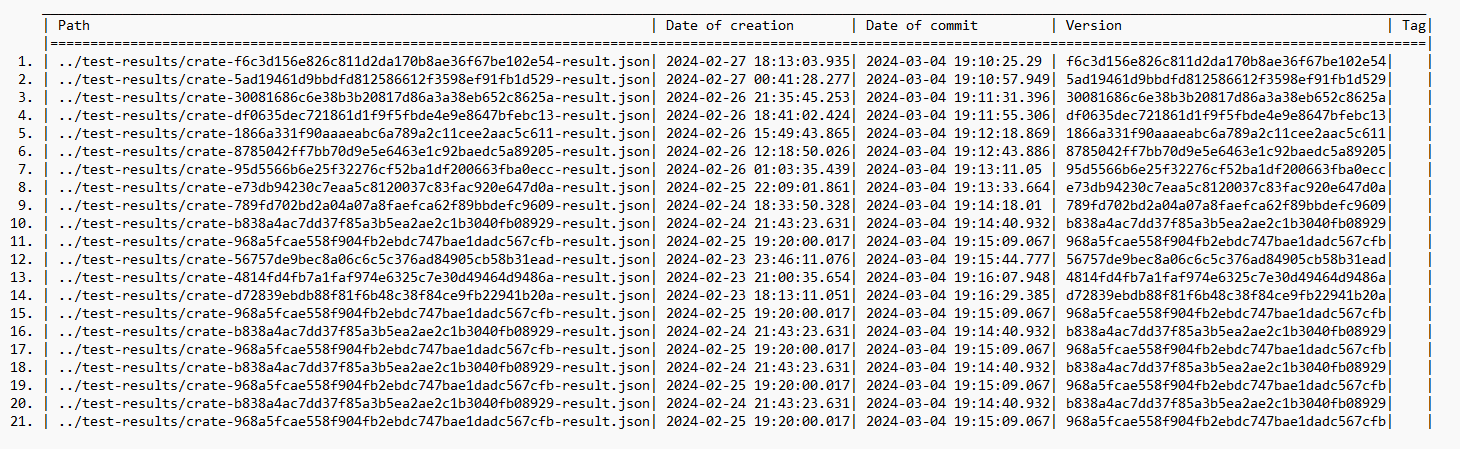
\includegraphics[width=1\textwidth]{../img/list-results-crate2.png}
    \caption{Obsah databáze systému PerfEval pro projekt crate se simulovanými záznamy}
\end{figure}

\begin{figure}[h!]
    \centering
    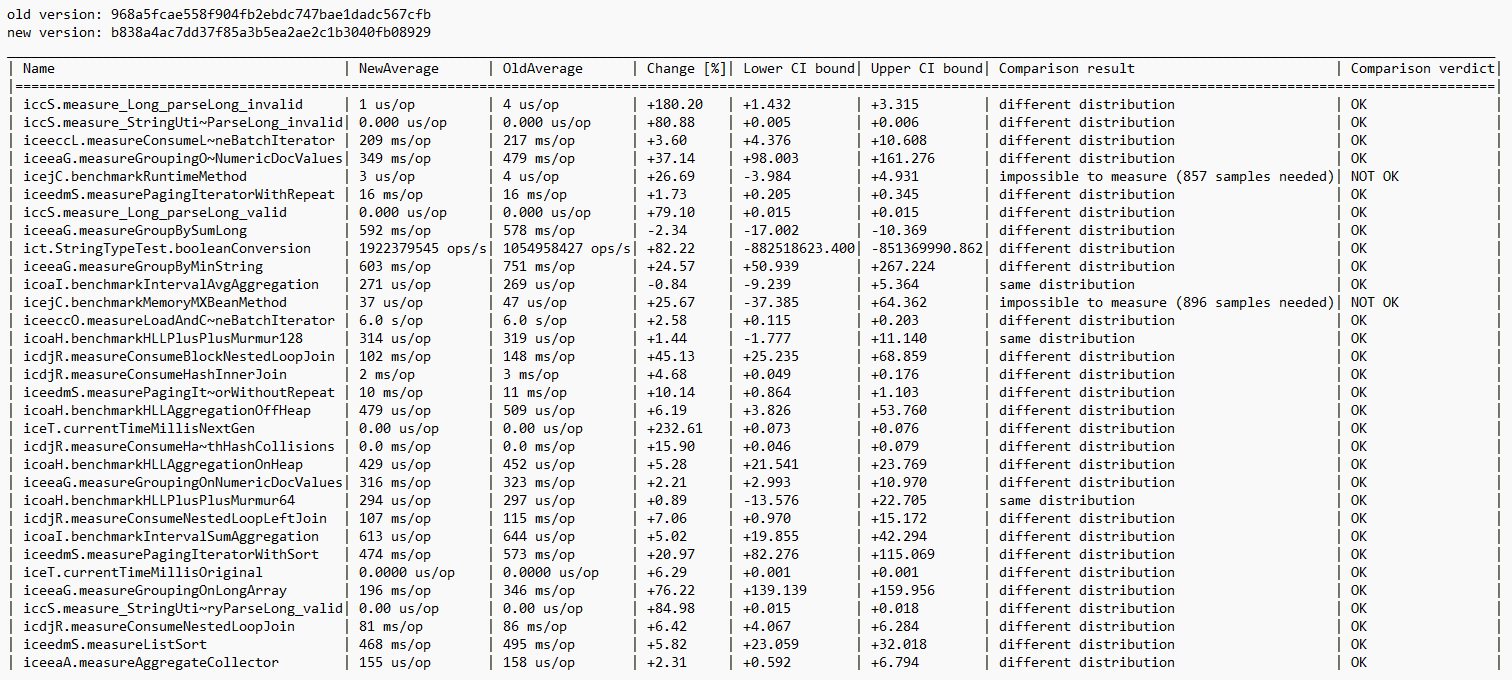
\includegraphics[width=1\textwidth]{../img/version-comparison-es.png}
    \caption{Výsledek porovnání po simulování měření}
\end{figure}

Výstup programu s nasimulovanými výsledky měření ukazuje, že výsledky není možné
doměřit. V~konfiguračním souboru je maximální počet měření, který lze provést shora omezen číslem 100.
Pokud tedy PerfEval odhadl, že by bylo zapotřebí více než 100 měření, tak selže (exit kód 1).
PerfEval tedy není schopen v~tomto případě sám o~sobě rozhodnout jestli se nová verze nezhoršila.
